\chapter{Understanding the functional impact of mTOR clinical kinase mutations using physical modeling}

\section{Gloss}

The work in this chapter touches and builds on work previously published. Some of the text in the methods section was published in the \emph{Journal of Clinical Investigation} in the following paper, and is reproduced with permission: 

\realsinglespacing
\flushleft{\bf Mechanistically distinct cancer-associated mTOR activation clusters predict sernsitivity to rapamycin}
\flushleft{{\bf Jianing Xu$^{1}$, Can G, Pham$^1$, Steven K. Albanese$^{2,3}$, Yiyu Dong$^1$, Chung-Han Lee$^1$, Vanessa Rodrik-Outmezguine$^4$, Zhan Yao$^4$, Song Han$^1$, David Chen$^5$, Daniel L. Parton$^3$, John D. Chodera$^{3,6}$, Neal Rosen$^{4,7}$, Emily H. Cheng$^{1,8,9}$, James J. Hsieh$^{1,7,10,*}$} \\
	\emph{\normalsize $^1$ Human Oncology and Pathogenesis Program, Sloan Kettering Institute, Memorial Sloan Kettering Cancer Center, New York, NY} \\
	\emph{\normalsize $^2$ Louis V. Gerstner, Jr. Graduate School of Biomedical Sciences, Memorial Sloan Kettering Cancer Center, New York, NY} \\
	\emph{\normalsize $^3$ Computational and Systems Biology Program, Sloan Kettering Institute, Memorial Sloan Kettering Cancer Center, New York, NY}\\
	\emph{\normalsize $^4$ Molecular Pharmacology Program, Sloan Kettering Institute, Memorial Sloan Kettering Cancer Center, New York, NY}\\
	\emph{\normalsize $^5$ Oncology Global Development, Novartis Pharmaceuticals Corp., East Hanover, NJ}\\
	\emph{\normalsize $^6$ Physiology, Biophysics, and Systems Biology Program, Weill Cornell Medical College, Cornell University, New York, NY}\\
	\emph{\normalsize $^7$ Department of Medicine, Memorial Sloan Kettering Cancer Center, New York, NY}\\
	\emph{\normalsize $^8$ Department of Pathology, Memorial Sloan Kettering Cancer Center, New York, NY}\\
	\emph{\normalsize $^9$ Department of Pathology and Laboratory Medicine,Weill Medical College of Cornell University, New York, NY}\\
	\emph{\normalsize $^{10}$ Department of  Medicine,Weill Medical College of Cornell University, New York, NY}\\
	\emph{\normalsize $^*$ Corresponding Author} \\
}
\realdoublespacing
\medskip

This chapter contains early attempts to understand the functional impact of missense mutations on the structure and function of mTOR, which plays a critical role in controlling cell growth and regulation. These mutations stand out because they are relatively rare, but occur in a large percentage of clear cell renal cell carcinoma case, which is often treated with an allosteric mTOR inhibitor. Further, these mutations occur in roughly 2\% of \emph{all} cancer patients, meaning many thousands of patients could be impacted by understanding the impact of these mutations. Understanding 

The challenges and frustration we encountered in this work, namely the shortcomings of traditional molecular dynamics analysis for providing mechanistic and testable hypotheses for explaining the hyperactivating phenotype caused by these mutations, inspired the shift in focus to more quantitative models that will be explored more deeply at the end of this chapter and for the entirety of Chapter 4 of this dissertation. While the research presented in this chapter is largely inconclusive, it highlights the importance of using physical modeling to predict experimentally testable, quantitative observables when trying to understand the impact of missense mutations. 

This work largely builds on the experimental work of Jianing Xu, James Hsieh and the rest of the authors from the publication highlighted above that identified and characterized the mutations that were studied computationally in this chapter. Importantly, this work identified the potential for multiple mechanisms of activation by these mutations, which is what motivated the computational studies on structure that followed. While this paper contains initial analysis of the calculations we performed, this chapter contains previously unpublished analysis of a larger, more complete dataset than was available for that publication. This chapter also contains preliminary calculations that I set up using FEP+ with advice from Kevin Hauser and Lingle Wang. 

\section{Introduction}
\subsection{mTOR forms the catalytic core of protein complexes that control a number of cellular processes}
mTOR (mammalian target of rapamycin) is a serine-threonine kinase that controls a number of cellular processes~\citep{Laplante:2012fm,Saxton:2017cv} by integrating signaling from the MAPK and PI3K pathways~\citep{Mendoza2011-bj}. mTOR forms the catalytic core of heteromeric protein complexes, mTORC1 and mTORC2, that differ in the regulatory proteins that decorate the kinase. mTORC1 is defined by RAPTOR~\citep{Kim:2002vh,Hara:2002tn} and PRAS40~\citep{Yang:2017gu}, while mTORC2 is characterized by RICTOR~\citep{Sarbassov:2004kv}. Each complex contains a number of shared regulatory proteins, such as mLST8~\cite{BarPeled:2012gq} and DEPTOR~\citep{Peterson:2009fc}. mTOR itself is an atypical kinase, and includes a number of insertions that deviate from the canonical kinase fold. The C-terminal fragment crystal structure (Figure~\ref{fig:mtor-figure1})shows that the kinase domain is hugged by a FAT domain~\citep{Yang:2013gaa}, forming a C-shaped clamp around the kinase domain. The FAT domain forms a number of regulatory salt bridges that have been implicated in controlling the activity of the kinase~\cite{Yang:2013gaa}. The FK506-rapamycin-binding (FRB) domain hangs over the opening cleft to the active site~\cite{Yang:2013gaa} (Figure~\ref{fig:mtor-figure1}). The FRB domain is exposed in mTORC1, while is it thought to be occluded and inaccesible to FKBP12 in mTORC2~\citep{Gaubitz:2015gr}. Complex activity is hypothesized to be regulated via restricted access to the active site by architectural elements as well as rapalog-mediated recruitment of FKBP to the FRB domain~\citep{Aylett:2016gs}. 

\begin{landscape}
	\begin{figure}[p]
		\centering
		\includegraphics[width=0.8\linewidth]{figures/mtor-fig1.pdf}
		\caption[mTOR is an atypical kinase with a number of regulatory domains]{
			{\bf mTOR is an atypical kinase with a number of regulatory domains}
			mTOR (PDBID: 4JSV) is shown as a cartoon diagram. The kinase domain (white) has a number of structural features highlighted, such as the activation loop (teal) as well as a network of regulatory $\alpha$ helices (red) in the active site. The FAT domain (black) clamps around the kinase domain and forms a number of salt bridge and hydrophobic contains with the kinase domain. The FRB domain (gold) hangs over the active site clef and is the site of rapalog binding and rapalog-mediate FBKBP recruitment. \bf{This figure reprinted with permission of James Hsieh}
		}
		\label{fig:mtor-figure1}
	\end{figure}
\end{landscape}

mTORC1 controls a number of biological processes by integrating multiple upstream signals (Figure~\ref{fig:mtor-figure2}). Tuberous sclerosis complex 1/2 (TCS1/2) integrates growth factor signaling from the PI3K/AKT pathway~\citep{Inoki:2002jv,Manning:2002tp} and DNA damage from AMPK~\citep{Jones:2005kg}. TSC1/2 acts as GTPase activating protein (GAP) for RHEB~\citep{Inoki:2003je}, which binds to and activates mTORC1 at the lysosomal surface. mTORC1 localization is controlled by the second major signal it integrates: amino acid availability. Upon stimulation by amino acids, the Ragulator~\citep{BarPeled:2012fr} recruits inactive mTORC1 from the cytosol to the lysosomal surface~\citep{Kim:2008kb,Sancak:2010bu,Efeyan:2012de}, enabling interaction with RHEB. Once active, mTORC1 controls cell growth and protein synthesis by phosphorylating and activating S6K at T389 and inactivating 4EBP1 via a phosphorylation at S65~\citep{Hay:2004ir,Laplante:2012fm}. mTORC1 also activates SREBP1/2, which regulates lipid biosynthesis~\citep{Lamming:2013dza}. mTORC1 activation inhibits autophagy through via ULK1. Recent work suggests that mTORC1 can also control the biophysical properties of the cytoplasm by regulating crowding~\citep{Delarue:2018ca}, impacting the rate of diffusion and expanding the already diverse array of essential processes that mTOR controls. 

\subsection{mTOR is the targeted by inhibitors with two distinct mechanisms of action}
Due to the central role mTOR plays in a wide array of biological processes, it has emerged as the target of extensive drug discovery programs. There are two distinct classes of inhibitors developed to target mTOR: ATP-competitive inhibitors and allosteric inhibitors~\citep{Ballou:2008ec,Lamming:2013kg}. Temsirolimus~\citep{Hudes:2007kp} and Evirolimus~\citep{Motzer:2008cn} are FDA-approved inhibitors~\citep{fda-approved-kinase-inhibitors} that are thought to inhibit mTOR through recruiting FKBP family members, such as FKBP12, to the FRB domain~\citep{Hausch:2013iu}. Evidence suggests FKBP12 recruitment may inhibit mTORC1 activity by inducing a conformational change that prevents S6K binding~\citep{Yip:2010bm}. Further incubation leads to destabilization and disassembly of the protein complex, which is consistent with the time-dependent nature of rapalog inhibition of mTORC1 mediated 4EBP1 phosphorylation~\citep{Yip:2010bm}. The rapalogs are potent inhibitors of mTORC1, while mTORC2 requires chronic rapalog treatment and is highly dependent on FKBP expression levels~\citep{Schreiber:2015fi}. A cryo-EM structure of TORC2 suggests that the FRB domain is inaccessible in TORC2, explaining the relative insensitivity of mTORC2 to rapalog inhibition~\citep{Gaubitz:2015gr}. Rapalogs have also been shown to only partially inhibit mTORC1, often failing to reduce 4EBP phosphorylation levels~\citep{Saxton:2017cv}, despite efficacy at preventing S6K phosphorylation. 
There are an array of ATP-competitive inhibitors developed to target mTOR and other members of the PI3K family of kinases, such as MLN0128~\citep{Slotkin:2015je,Hassan:2014kl}, INK-228 (TAK-128)~\citep{GarciaGarcia:2012jc}, AZD8055~\citep{Chresta:2010ir}, PKI-587~\citep{Mallon:2011gn}, and BEZ-235~\citep{Mukherjee:2012ki}. ATP-competitive inhibitors exhibit a wide range of selectivity, with many inhibiting mTORC1, mTORC2, and multiple isoforms of PI3K. ATP competitive inhibitors target the catalytic activity of mTOR and more fully inhibit mTORC1 and mTORC2 phosphorylation of downstream targets~\citep{Saxton:2017cv}. While many of these inhibitors have struggled clinically due to modest clinical benefits and high toxicity leading to low tolerability~\citep{Pongas:2016jm}, there is considerable excitement about developing mTOR inhibitors to treat a number of diseases. ATP-competitive inhibitor BEZ-235 has shown promising results in preclinical models of lapatinib-resistant PI3K hyperactivated breast cancer~\citep{Eichhorn:2008ff}.  Dual targeted catalytic inhibitors that target both PI3K and mTOR have shown success by abrogating reactivation of Akt, which is caused by the alleviation of negative feedback due to long term treatment with mTOR inhibitors~\citep{RodrikOutmezguine:2011fb}. For example, a dual-inhibitor of mTORC and PI3K$\alpha$, PI-103, showed promising activity against glioma xenografts~\citep{Fan:2006kw}. 

mTOR inhibitors show the most promise in treating diseases with mTOR pathway alterations pathway~\citep{Wagle:2014ej}. Despite initial success, resistance mutations in the FRB or kinase domain have been observed~\citep{Wagle:2014be}. Work has also been done to combine the two mechanisms of action in Rapalink-1, which tethers rapamycin and MLN0128~\citep{RodrikOutmezguine:2016km} with a flexible linker and overcome such acquired resistance. Rapalink also shows improvements over ATP-competitive inhibitors or rapalogs outside of the context of resistance.  In glioblastoma models, ATP-competitive inhibitor MLN0128 and allosteric inhibitor rapamycin showed poor \emph{in vivo} efficacy. In contrast, RapaLink-1, by overcoming poor residence time and potency, was able to durably inhibit mTORC1 and cross the blood-brain barrier~\citep{Fan:2017fk}. 

\begin{landscape}
	\begin{figure}[p]
		\centering
		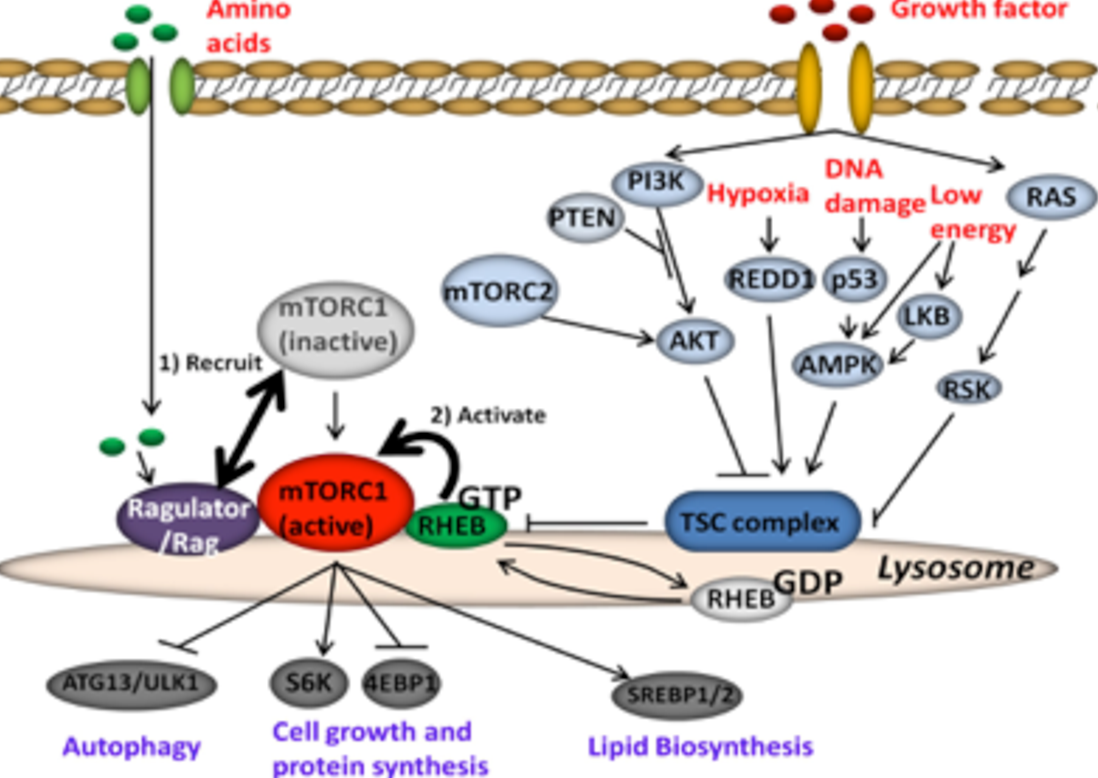
\includegraphics[width=0.8\linewidth]{figures/mtor-fig2.pdf}
		\caption[mTORC1 integrates signaling from a number of inputs]{
			{\bf mTORC1 integrates signaling from a number of inputs}
			The signaling pathway of mTOR involves integrating signaling from the growth factors, amino acids, hypoxia, and DNA damage. Integrating such signals controls the localization and activity of mTORC1, which controls autophagy, cell growth, and macromolecule synthesis through phosphorylation of downstream targets. \bf{This figure courtesy of James Hsieh} 
		}
		\label{fig:mtor-figure2}
	\end{figure}
\end{landscape}

\subsection{mTOR signaling is dysregulated in cancer by hyperactivating missense mutations}
mTOR pathway alterations have been observed in a wide array of cancer types~\citep{Guertin:2007dw} and extensively characterized. Less well studied are missense mutations in mTOR itself. An exceptional responder in a phase 1 clinical trial of pazopanib and everolimus with metastatic urothelial carcinoma lead to the identification of two missense mutations in mTOR~\citep{Wagle:2014ej}, E2014K and E2419K. Subsequent work identified 33 MTOR mutations gathered from publicaly available tumor sequencing data, and found that a number of them activated the mTOR pathway and conferred sensitivity to mTOR inhibitors when engineered into various cancer cell lines \emph{in vitro}~\citep{Grabiner:2014be}. While these missense mutations are pulled from an array of different cancer types, mTOR missense mutations have been observed in about 15\% of clear cell renal cell carcinoma~\citep{CancerGenomeAtlasResearchNetwork:2013ib}. Characterization of these mutations revealed that not only do many of these mutations hyperactivate mTOR (Figure ~\ref{fig:mtor-figure3}), but they can be grouped into complementation groups by determining which double mutations cause hyperactivation at levels higher than the constituent single mutants alone~\citep{Xu:2016fw}. This suggests that these mutations can activate mTOR through different, seemingly complementary mechanisms. 

\begin{landscape}
	\begin{figure}[p]
		\centering
		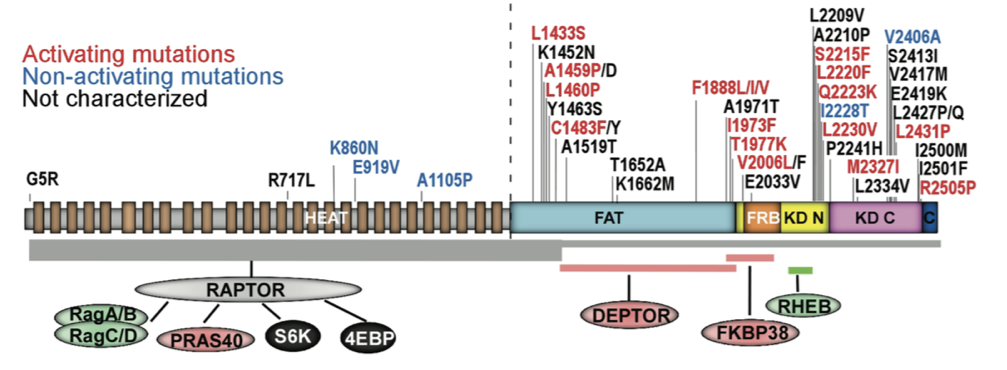
\includegraphics[width=1.0\linewidth]{figures/mtor-fig3.png}
		\caption[Hyperactivating mTOR missense mutations have been observed in cancer]{
			{\bf Hyperactivating mTOR missense mutations have been observed in cancer}
			Diagram shows the domain structure of mTOR, its regulatory interaction partners (negative regulators in pink, positive regu- lators in green, and a dual-role regulator in gray), and the substrates of mTORC1 complex. The positions within mTOR that are involved in the interaction with the regulatory partners are highlighted below the domain structure. The thickness of the horizontal bar of RAPTOR-mTOR interaction indicates the relative binding affinity. mTOR missense mutations derived from ccRCC are mapped and color coded
			to summarize their respective effects on mTORC1 signaling (activating mutations in red). KD N, kinase domain N lobe; KD C, kinase domain C lobe. \bf{This figure reprinted with permission of James Hsieh and the Journal of Clinical investigation~\citep{Xu:2016fw}.}
		}
		\label{fig:mtor-figure3}
	\end{figure}
\end{landscape}

\subsection{Using physical modeling to understand the functional impact of mTOR mutations}
To begin to understand the impact of these missense mutations at an atomistic level, we performed massively parallel molecular dynamics~\citep{Salsbury:2010ij} using the computing resource Folding@Home~\citep{Shirts:2000du}. Molecular Dynamics simulations have been used previously to understand the mechanism of oncogenic and resistance mutations on the structure and activation of EGFR~\citep{Shan:2012bs,Sutto:2013gy}. They have also been applied to understanding missense mutations in p53~\citep{Demir:2011bc}, CLIC2~\citep{Witham:2011co}, opsin~\citep{Tsukamoto:2013gr}, and a host of oncogenes and tumor suppressors\citep{Stehr:2011ga}. Using the previously solved crystal structure~\citep{Yang:2013gaa}, we built models for 45 single, and 190 double mutations, far more than could be crystallized individually~\citep{Xu:2016fw}. We analyzed the simulations for changes in contact formation, as well as changes in order parameters for activation mined from other kinase studies and previous work on mTOR biochemistry. We also piloted alchemical free energy calculations~\citep{Chodera:Curr.Opin.Struct.Biol.:2011} on a number clinically observed mutants, to compute physical, testable properties such as change in affinity for ATP-competitive inhibitors and ATP itself. In doing so, we identify promising candidates for resistance mutations to an ATP competitive inhibitor, and lay the ground work for future studies on the application of these methods to studying the functional impact of mutations on inhibitor binding. Taken together, this work forms the beginning of a comprehensive analysis of the impact of these mutations on structure and small molecule binding, which has implications for the treatment of patients with these mutations. 

\section{Results}

\subsection{Missense mutations perturb the structure of mTOR kinase domain}
To begin understanding the types of rearrangements missense mutations can induce in the local structure of mTOR, we employed contact map analysis to identify regions in which we detected changes in the formation of contacts from the wild type to mutant simulations. This is analysis is described in depth in the methods section. Briefly, we first calculated the distance between every residue pair based on the closest heavy atoms in each frame of the simulations after 100 ns. For each residue pair, we calculated the probability of forming a contact across all of the simulation data and replicas, using 5 $\AA$ as the threshold at which a contact was formed. The wild-type probability was subtracted from the mutant, giving a net change in probability to form a contact for each residue pair in the protein. This analysis was performed only for the kinase domain simulations, as the full contact map for the full length C terminal fragment was too computationally intensive to compute for the 190 mutant simulations. Using these maps, it is possible to identify regions in which the mutant is causing a conformational change, both locally near the mutant and more distantly through some allosteric mechanism. As an example of the 45 different mutant kinase domain simulations, we show the kinase domain simulations of S2215F, a highly activating and recurrent missense mutation~\citep{Xu:2016fwu}. S2215F shows evidence of a rapid, mutation-induced local rearrangement, causing disruption of the $\alpha$-helix in which it occurs (Figure~\ref{fig:mtor-figure4}, region 1). This unfolding is evident in many of the replicates, shown in red in the region 1 panel highlighted by Figure~\ref{fig:mtor-figure4}. S2215F, shown in yellow in Figure~\ref{fig:mtor-figure4}, also causes unwinding and loosening of $\alpha$-helix k$\alpha$8, despite this secondary structural element being far from where the mutant occurs (Figure~\ref{fig:mtor-figure4}, region 2). 


\begin{landscape}
	\begin{figure}[p]
		\centering
		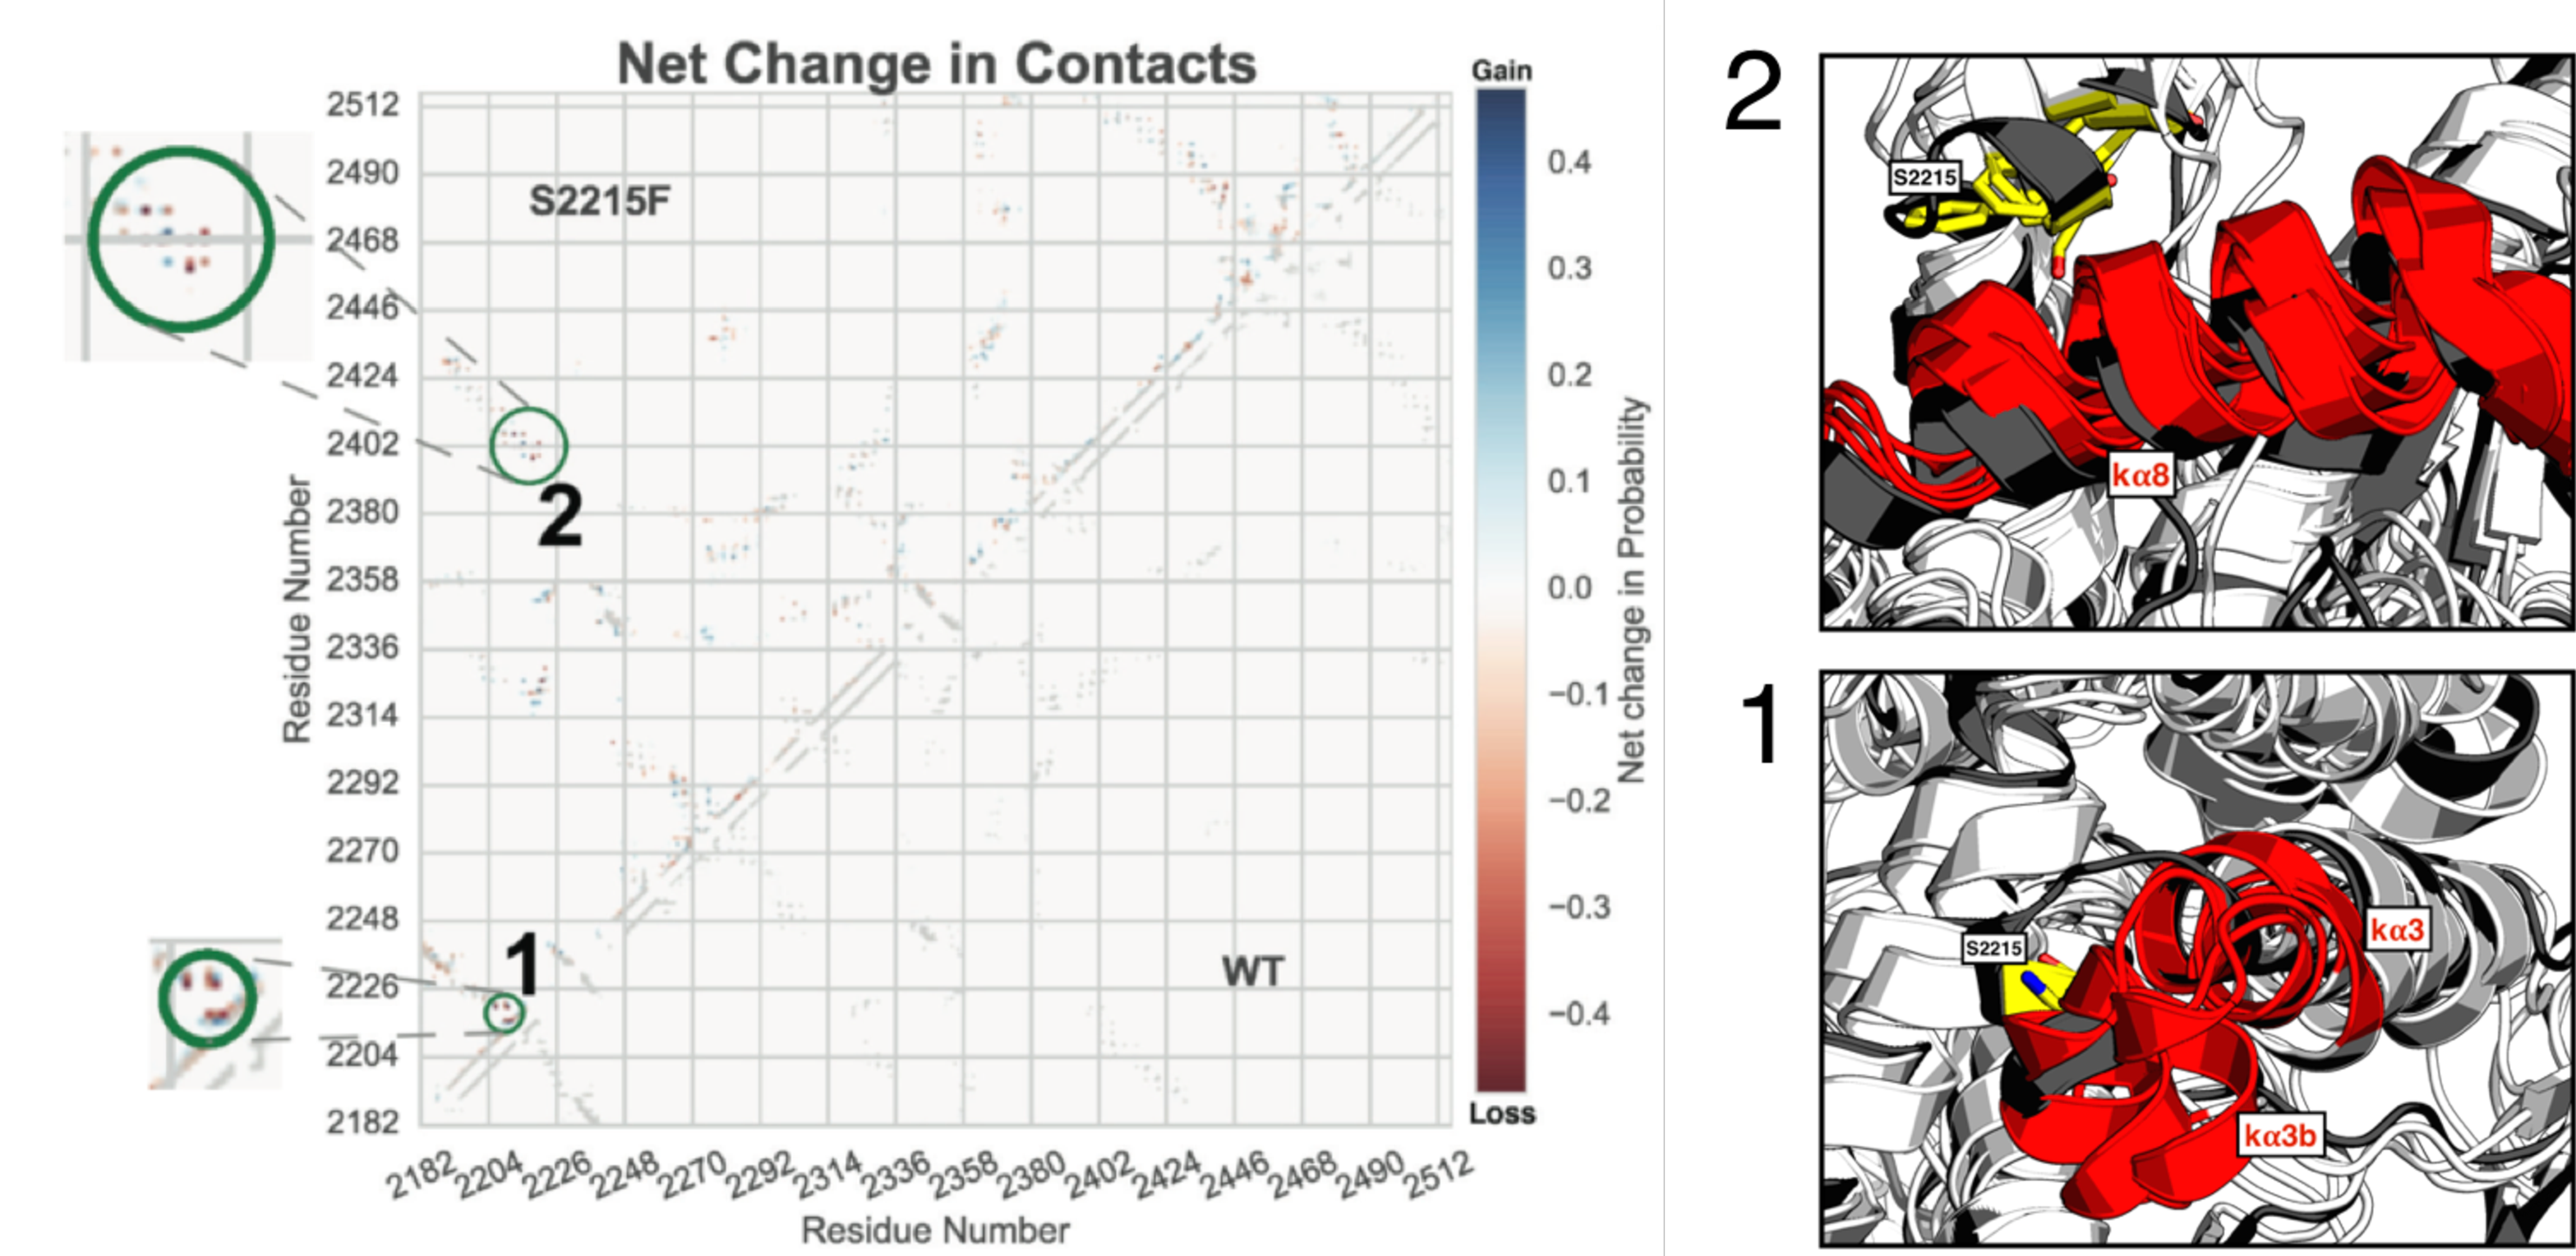
\includegraphics[width=1.0\linewidth]{figures/mtor-fig4.pdf}
		\caption[Missense mutations can perturb local structure]{
			{\bf Missense mutations can perturb local structure}
			{\bf Left} Contact map showing the difference in probability of forming a contact between WT and mutant S2215F for the kinase domain simulations. {\bf Right} Regions one and two highlighted in contact map, showing a structural perturbation in indicated helices. Starting structure is shown in gray, the residues indicated in the contact map are shown in red and residue 2215 is shown in yellow. All trajectories started from PDB: 4JSN. \bf{This left panel of this figure is a modified version of a figure that appears in~\citep{Xu:2016fw}. Reprinted with permission of James Hsieh and the Journal of Clinical investigation}
		}
		\label{fig:mtor-figure4}
	\end{figure}
\end{landscape}

\subsection{Missense mutations do not appear to shift the formation of an active kinase domain}

Despite the promise of being able to identify structural rearrangements in an automated, high-throughput fashion, contact map analysis is difficult to use to explain mechanistically how these mutants are activating. Seeking a more mechanistic understanding of how these mutants are activating, we looked at a common order parameter for activation from previous work on kinases~\citep{Shukla:2014jp}. In most kinases, there is a highly conserved lysine residue that coordinates ATP when it is bound in the active site. In mTOR, this lysine has been identified as K2187~\citep{Yang:2013gaa}. To test whether mutations are activating mTOR by shifting the kinase domain into a more active conformation, we looked at the contact formation over time between resides K2187-E2190 (indicative of an active kinase), shown in Figure~\ref{fig:mtor-figure5} in red, and E2190-R2430, shown in Figure~\ref{fig:mtor-figure5} in blue. We hypothesized that formation of the E2190-R2430 contact suggests an inactive kinase domain, as the $\alpha$C would need to rotate out and away from the active site, which has been observed in inactive kinases in previous work (Figure~\ref{fig:mtor-figure5}, inset panel)~\citep{Shukla:2014jp,Jura:2011eh}. Show on the right in Figure~\ref{fig:mtor-figure5} is a representative panel of the activating mutants from the kinase domain simulations, as well as the control wild type. While some of the mutants seem less stable than the wild type, none of them appear to shift the distribution of the kinase domain further towards formation of the K2187-E2190 contact, indicative of activation. This is likely because the mTOR kinase domain adopts an active conformation in all of the available crystal structures, and the simulations largely stay in the local minima of the crystal structure. This is further supported by the hypothesis that the mTOR kinase domain is constitutively active, and is regulated by restriction of substrate access~\citep{Yang:2013gaa,Laplante:2012fm,Saxton:2017cv}. 

\begin{landscape}
	\begin{figure}[p]
		\centering
		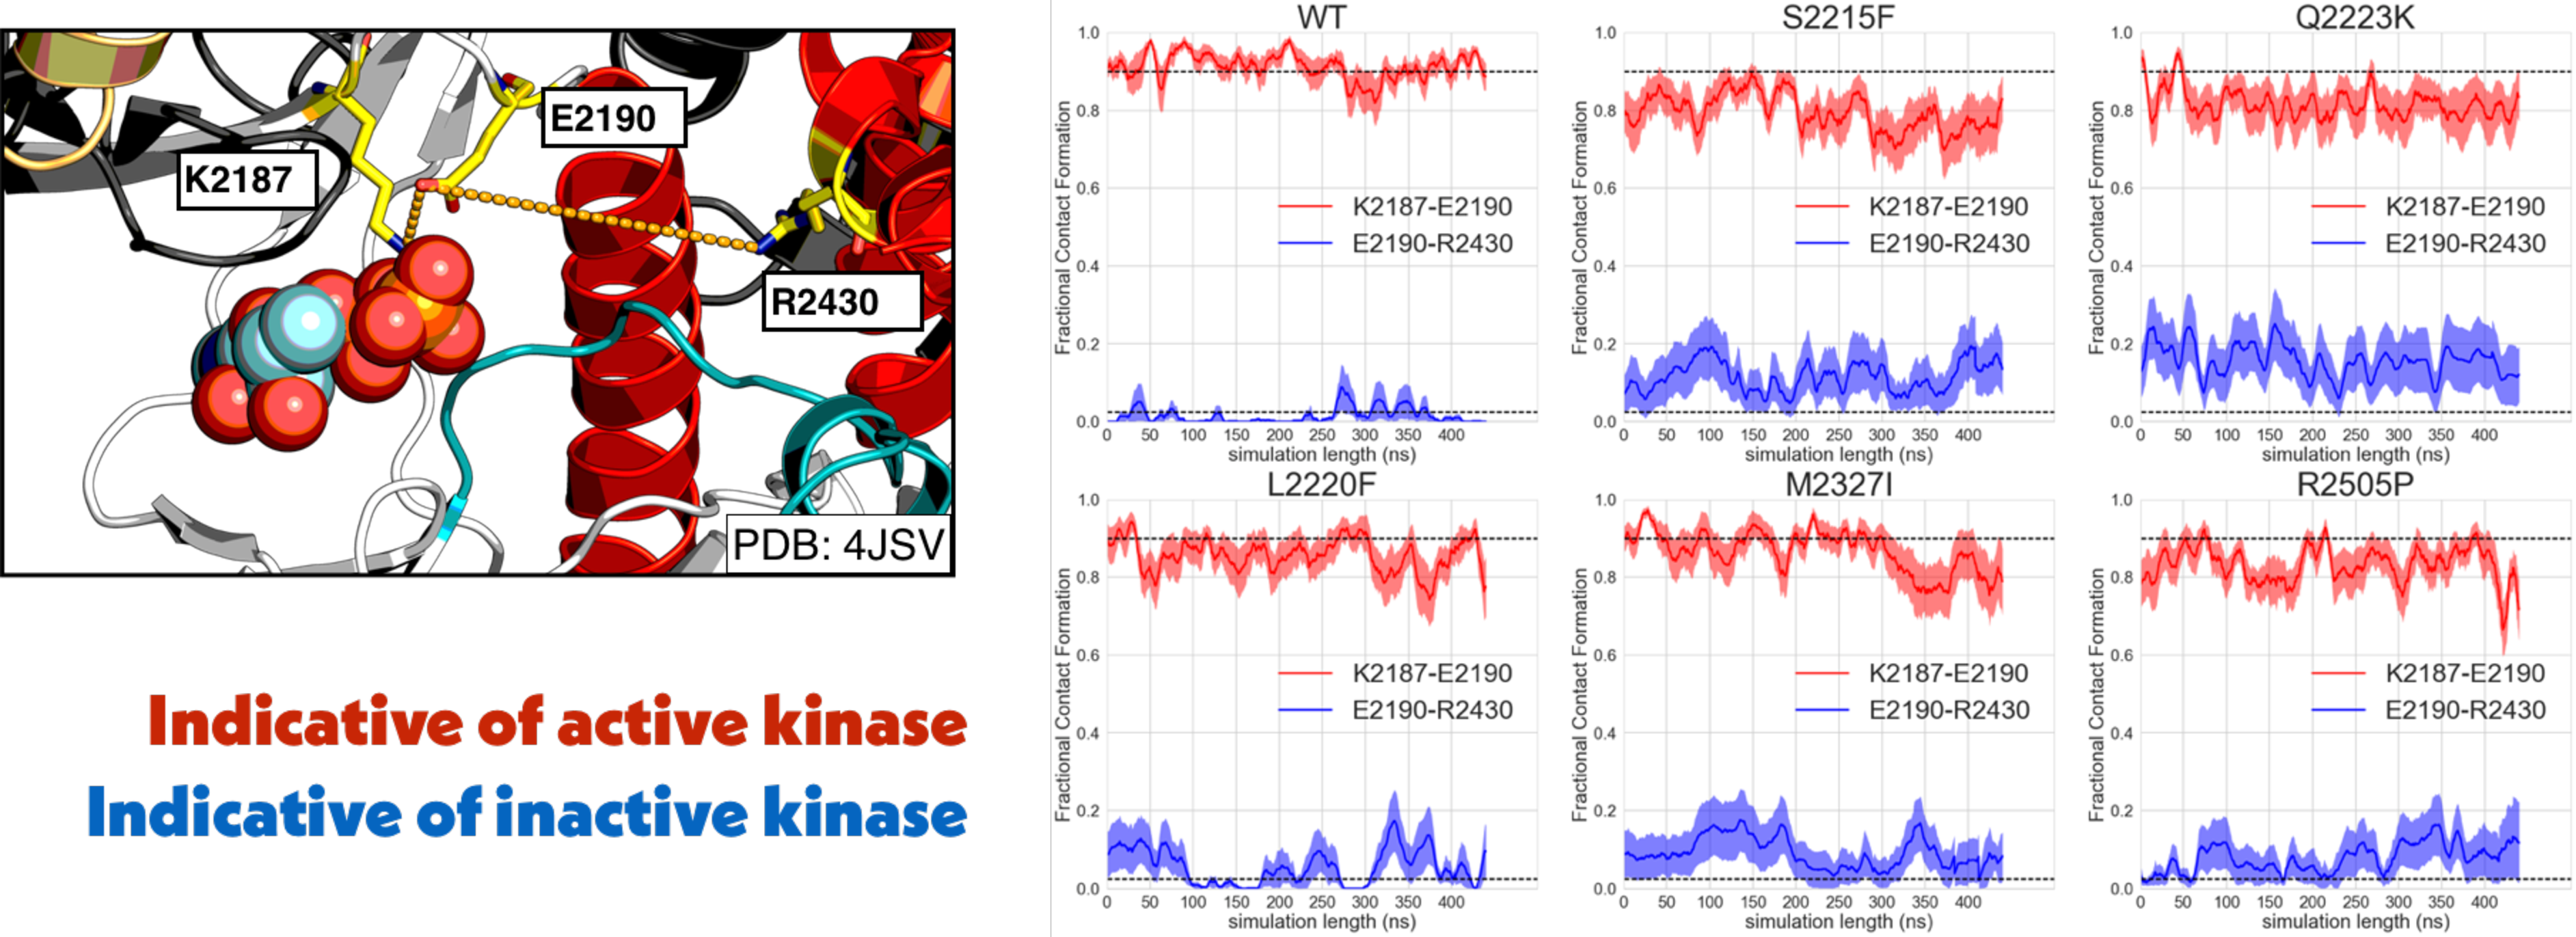
\includegraphics[width=1.0\linewidth]{figures/mtor-fig5.pdf}
		\caption[Missense mutations do not shift the population of the active conformation on a common activation order parameter]{
			{\bf Missense mutations do not shift the population of the active conformation on a common activation order parameter}
			{\bf Right} Fractional contact formation analysis for 20 500ns trajectories, analyzed in 20ns sliding window chunks. Contacts cutoff at 4Å for closest heavy atom.  Plotted is the mean $\pm$ SEM. The dashed lines represent the proportion roughly populated in the WT simulations. {\bf Left} Illustration of the bond formed between K2187 and E2190 (red) or E2190 and R2430 (blue). ATP is shown in spheres. The kinase domain (white) is shown with the activation loop (teal) and the $\alpha$ helices (red). The FRB domain is shown in gold. 
		}
		\label{fig:mtor-figure5}
	\end{figure}
\end{landscape}


\subsection{Missense mutations do not disrupt the formation of inhibitory salt bridges between the kinase and FAT domains}
Another hypothesis for how the missense mutations may be hyperactivating looked at the role the FAT domain, which clamps around the kinase domain, plays in regulating the activity of mTOR. In previous work, point mutations that disrupted the formation of the salt bridge between E2419 and R1905 (Figure~\ref{fig:mtor-figure6}, red) activated TOR signaling in yeast and mammalian cell lines~\citep{Urano:2007er}. From this observation, we hypothesized that stable contacts formed between the kinase domain and FAT domain have a negative regulatory role on the activity of mTOR, and that disruption of these bonds through some allosteric mechanism would allow an oncogenic mutant to activate mTOR. Another set of contacts, Gln1941 to Gln2200 (Figure~\ref{fig:mtor-figure6}, blue) is conserved across many mTOR orthologs~\citep{Yang:2013gaa}, suggesitng a potential regulatory role. We also looked at several other salt bridges in the vicinity of these contacts: E1147 and K2218 (cyan), Q1425 and R2322 (magenta), and E1427 and R2322 (yellow). Shown in Figure~\ref{fig:mtor-figure6} is a representative selection of mutations from the kinase domain, demonstrating that none of the salt bridges showed a prominent change from the wild type to mutant simulations. Of note, R2505P appears to have a disruption int he formation of the Q1941 and Q2200,  E1147 and K2218, and E2419 and R1905 contacts, indicating that this may be a possible mechanism of activation for this mutant. However, this is difficult to say with certainty without functional experimental data or additional computation to confirm this result. 

\begin{landscape}
	\begin{figure}[p]
		\centering
		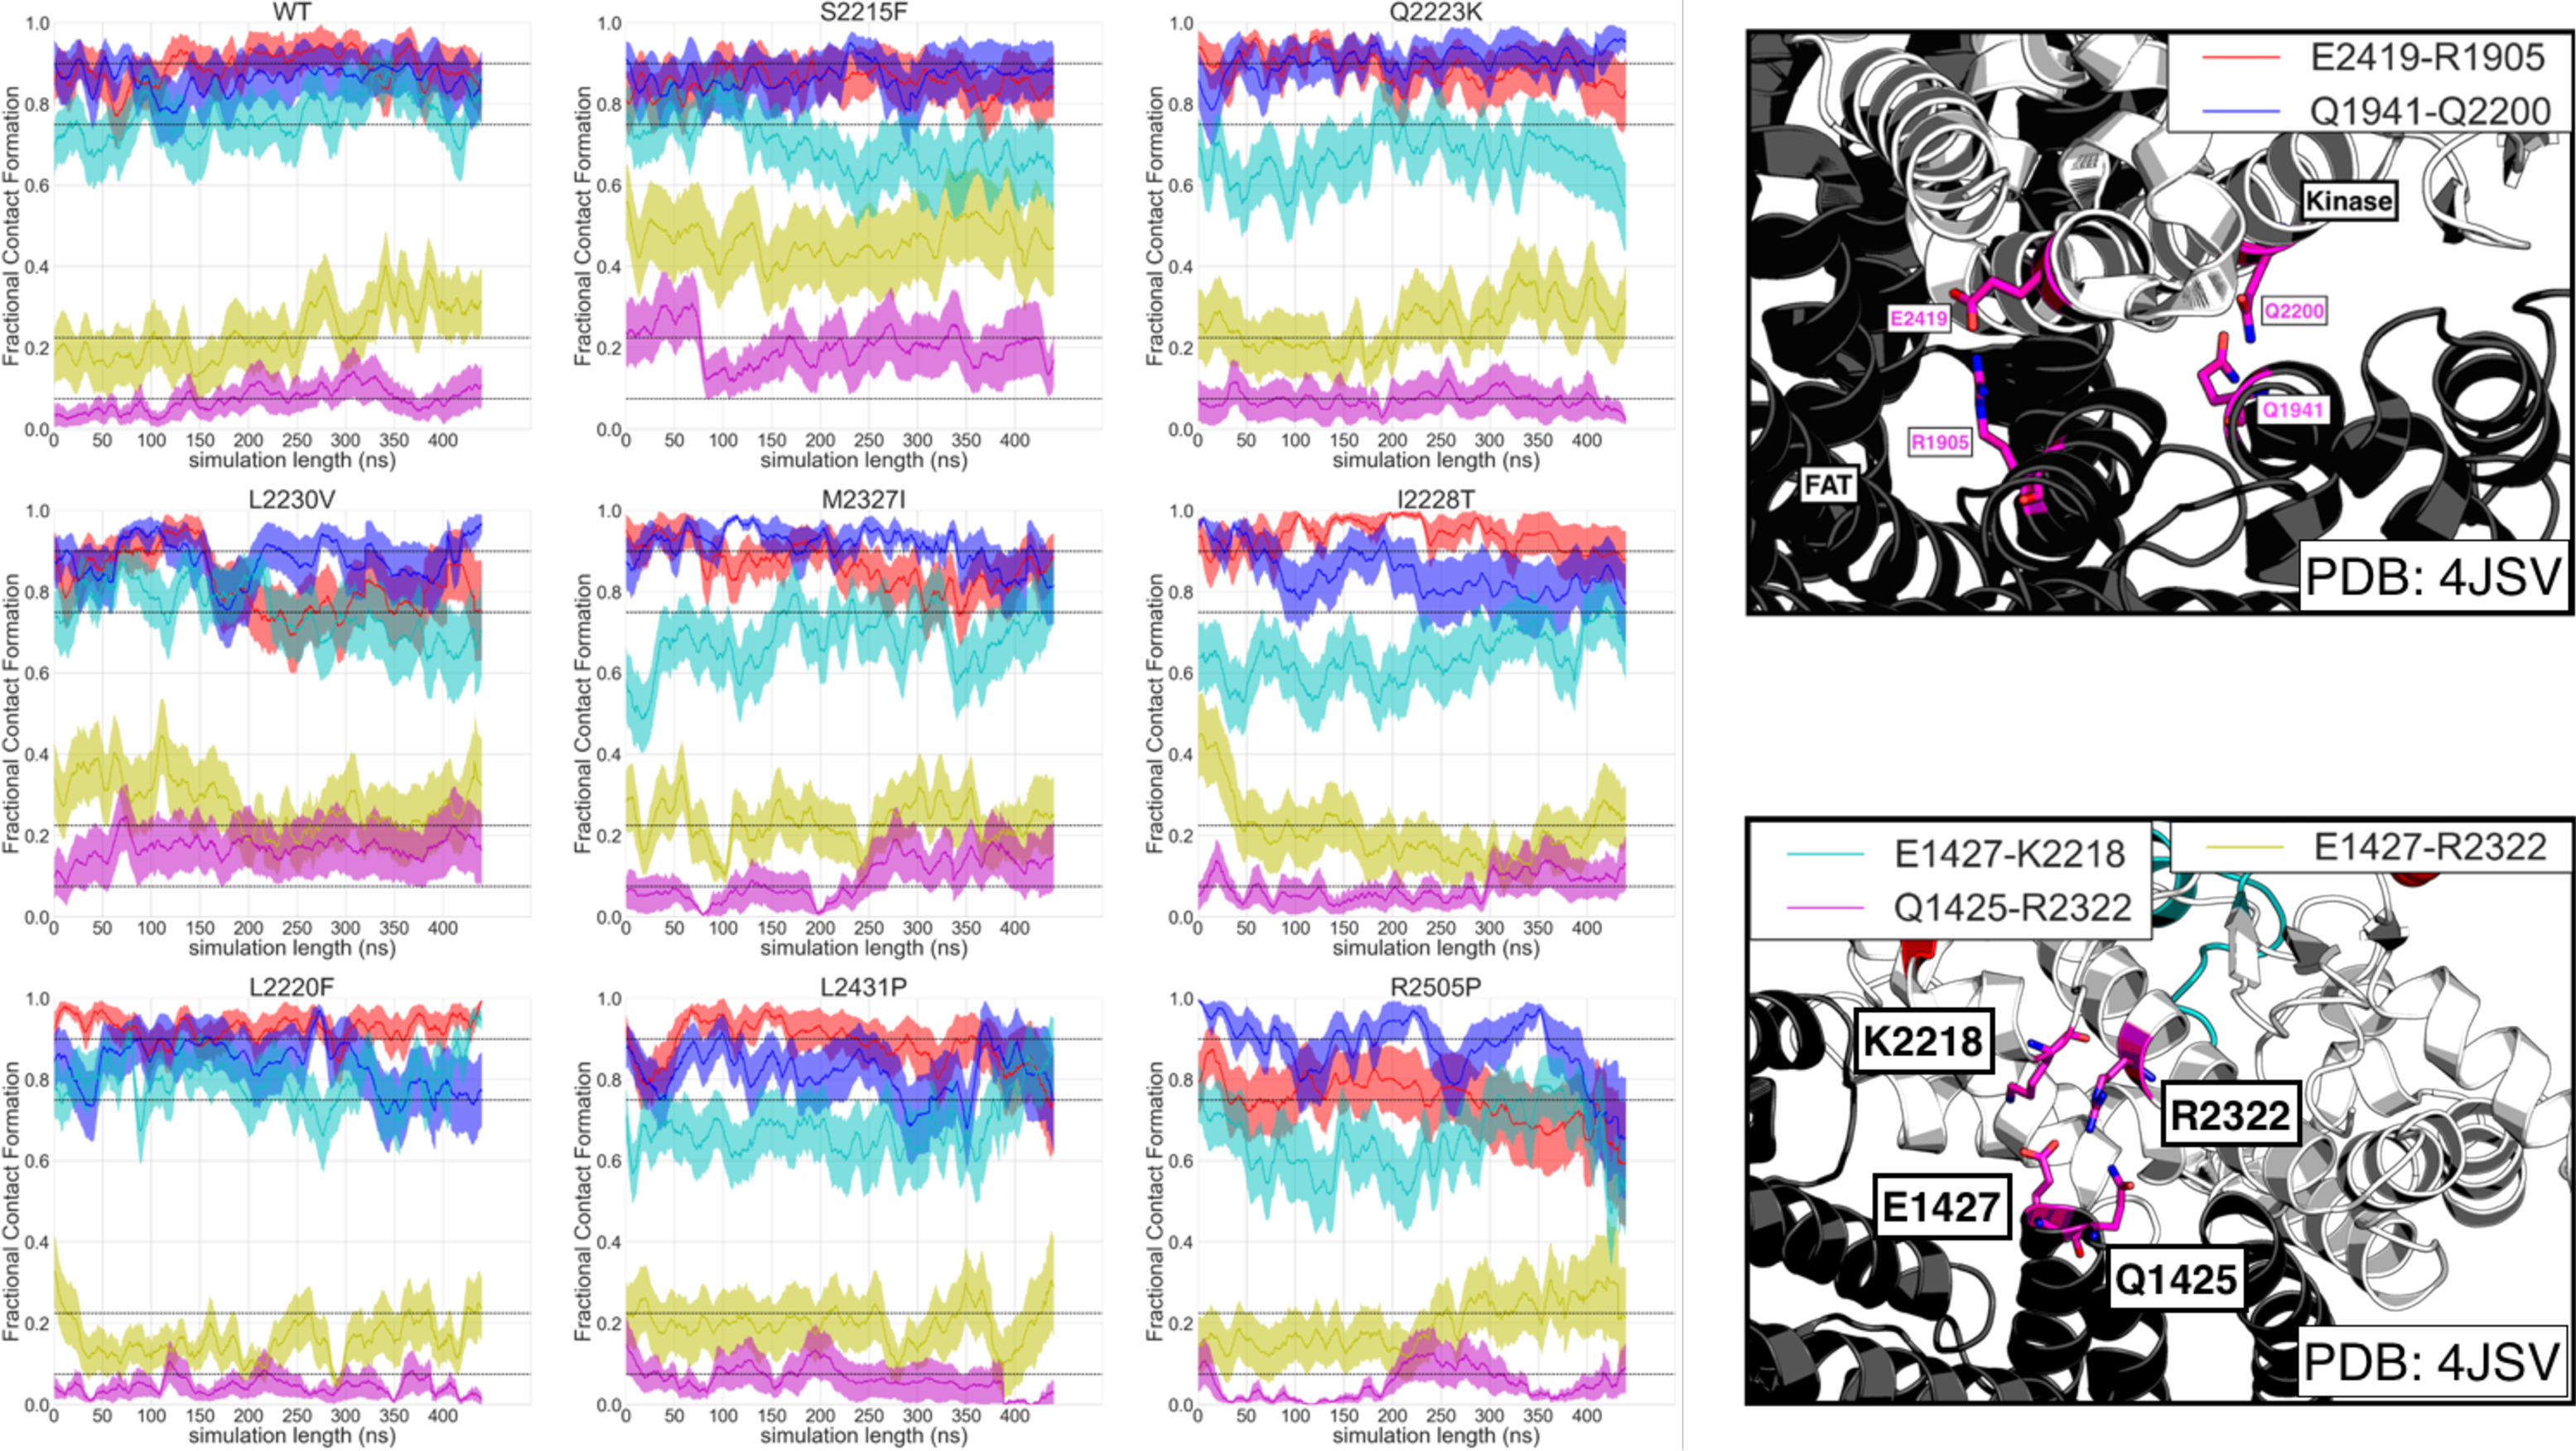
\includegraphics[width=1.0\linewidth]{figures/mtor-fig6.pdf}
		\caption[Missense mutations in kinase domain do not disrupt interactions between the kinase and FAT domains]{
			{\bf Missense mutations in kinase domain do not disrupt interactions between the kinase and FAT domains}
			{\bf Left} Fractional contact formation analysis for 10 500ns trajectories, analyzed in 20ns sliding window chunks. Contacts cutoff at 4Å for closest heavy atom.  Plotted is the mean $\pm$ SEM. The dashed lines represent the proportion roughly populated in the WT simulations. {\bf Right} Illustration of the distances being plotted between E2419 and R1905 (red), Q1941 and 2200 (blue), E1147 and K2218 (cyan), Q1425 and R2322 (magenta), or E1427 and R2322 (yellow). The kinase domain (white) interacts with the FAT domain (black) through salt bridges and hydrogen bonds formed by the highlighted residues (magenta) 
		}
		\label{fig:mtor-figure6}
	\end{figure}
\end{landscape}

\subsection{Free energy calculations show promise in predicting impact of mutations on small molecule and ATP affinity}
The preceding work on trying to understand the functional impact of mutations using traditional molecular dynamics highlights one of the key challenges of the application of physical modeling to this question: the need to compute meaningful, physically testable quantities. Alchemical free energy calculations have been previously used to predict the impact of mutations on protein-protein binding~\citep{clark2017free} and protein thermostabilities~\citep{steinbrecher2017predicting}. Based on this work, we set out to see if free energy calculations could be used to identify clinically observed mutations that might cause resistance to an ATP-competitive inhibitor. Here, we propose a model of resistance mutants that cause a decrease in affinity for an ATP-competitive inhibitor while maintaining a basic level of ATP affinity (Figure~\ref{fig:mtor-figure7}, left panels). An increase in ATP affinity could be a mechanism of resistance by making it more difficult for ATP-competitive inhibitors to out-compete ATP, as well as a mechanism of activation. To explore the impact of mutations on affinity for these compounds, we built models of mTOR bound to ATP (Figure~\ref{fig:mtor-figure7}, top left) and AZD8055 (Figure~\ref{fig:mtor-figure7}, bottom left). Using protein mutation FEP+~\citep{Hauser:2018vz,steinbrecher2017predicting}, we ran preliminary calculations for a small panel of mutations from the MSKCC-IMPACT assay~\citep{Zehir:Nat.Med.:2017}. Three showed greater than 1-log unit, or 1.4 kcal/mol, decrease in affinity for AZD8055 (Figure~\ref{fig:mtor-figure7}, blue bars). W2239C, a missense mutation observed in a patient with cervical squamous cell carcinoma that occured together with a known activating mutation S2215F~\citep{Cerami:2012eu,Gao:2013kd},  showed the greatest decrease in affinity (shown as a positive $\Delta \Delta G_{mutation}$ in Figure~\ref{fig:mtor-figure7}). While we were not able to confirm via prediction that ATP-affinity is not maintained, this result suggests that treatment with an ATP-competitive inhibitor targeting mTOR may be less effective than expected. M2345V and Y2225C are also both predicted to decrease the affinity for AZD8055. M2345V was observed in a cell line from a patient with cancer of unknown primary tissue and co-occurred with a TSC2 E75K mutation, which is likely to be loss of function~\citep{Barretina:2012fp}. Y2225C was observed in a patient with tubular stomach adenocarcinoma, who also had a slight copy number gain in both MTOR and DEPTOR~\citep{CancerGenomeAtlasResearchNetwork:2017fh}. All three of these mutations are exceedingly rare and occur in tumors with relatively high mutation burden. These preliminary results suggest that free energy calculations can potentially aid in understanding or teasing apart the functional impact of rare mutations in complex tumors.

\begin{landscape}
	\begin{figure}[p]
		\centering
		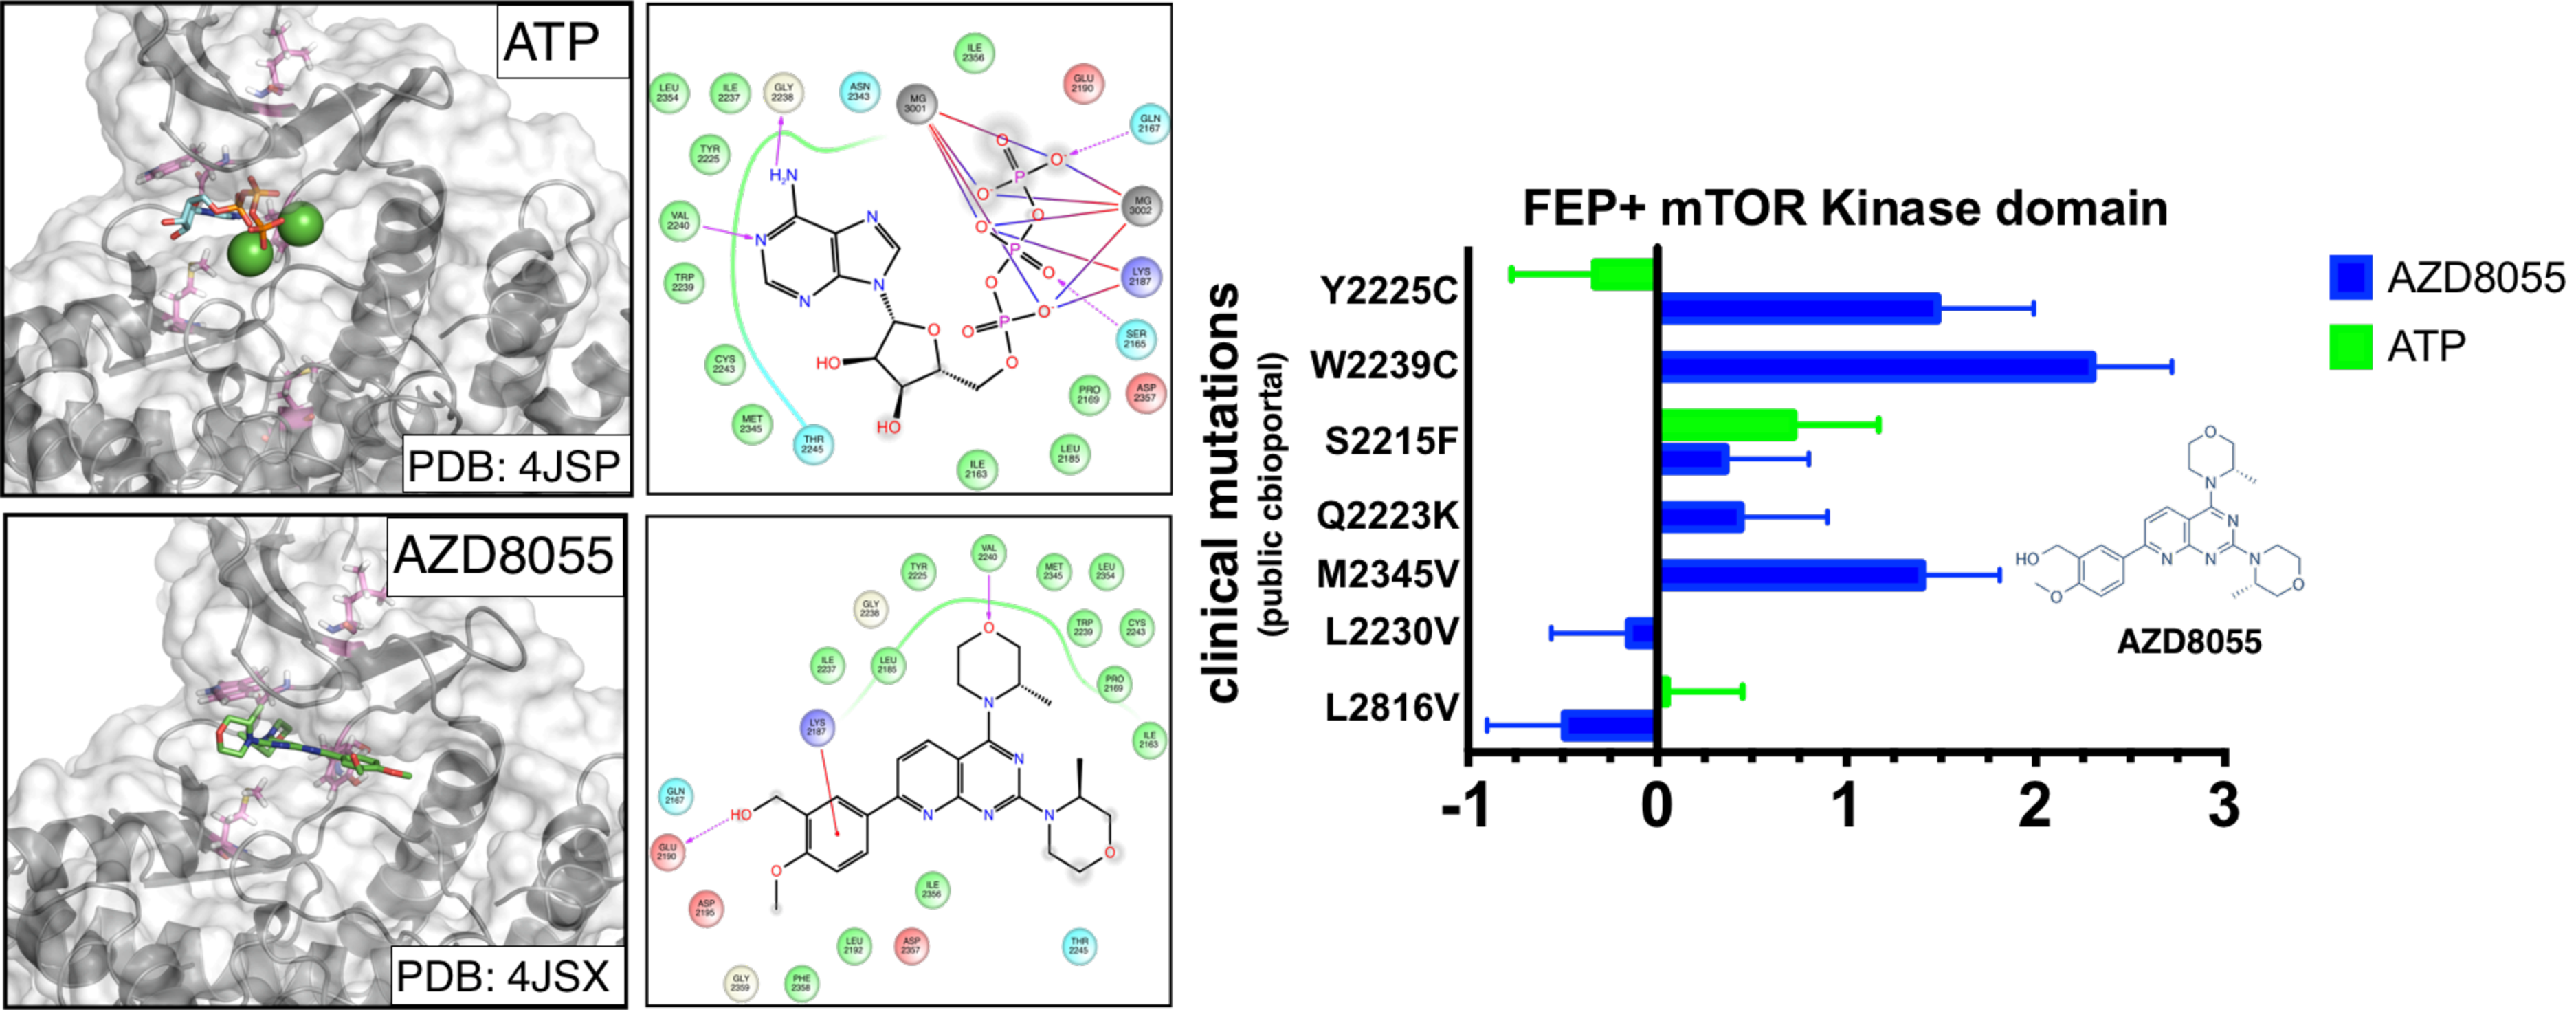
\includegraphics[width=1.0\linewidth]{figures/mtor-fig7.pdf}
		\caption[Free energy calculations identify potential resistance mutations]{
			{\bf Free energy calculations identify potential resistance mutations}
			{\bf Left} Structures and 2D interactions maps of ATP (top, PDBID: 4JSP) and AZD8055 (bottom, PDBID: 4JSX) docked to the kinase domain of mTOR. Magnesium ions are shown as green spheres.  {\bf Right} $\Delta \Delta G_{mutation}$ (x-axis) calculated for a number of clinically observed mTOR mutations(y-axis)~\citep{Zehir:Nat.Med.:2017} for ATP (green) and AZD8055 (blue). Error bars correspond to the BAR uncertainty estimate. 
		}
		\label{fig:mtor-figure7}
	\end{figure}
\end{landscape}


\section{Discussion and Conclusions}
The above work utilizes physical modeling to study the impact of clinically observed mutations on mTOR structure, function and ligand binding. mTOR is a critical node in multiple signaling pathways with a complex structure and regulatory.  Extensive molecular dynamics simulations were run on mutations that were confirmed to be hyperactivating by cellular and functional assays~\citep{Xu:2016fw}. Contact map analysis suggests that local, fast structural rearrangements are induced by mutations such as S2215F. Unfortunately, more focused studies on order parameters of activation do not yield insight into potential mechanisms of activation, suggesting that either the simulation time is insufficient to observe changes in the activation state of the kinase domain or the mechanism of activation occurs at the level of mTORC or substrate access. These studies are also limited by the relative scarcity of biophysical data for mTOR. At the time of the study, there were no atomistic structures for the mTOR complexes, impeding any study of the role mTOR mutations play in disrupting or altering the structure of the complex. Recent, exciting work using Cryo-EM has yielded a number of high resolution structures for mTORC1 and mTORC2~\citep{Yang:2017gu,Stuttfeld:2018kg,Yuan:2016ef,Yang:2016kk}. These advances would enable future work exploring the impact of mutations in the more physiologically relevant context of the complexes. Additionally, a more thorough understanding of the activation state of the mTOR crystal structure, which is assumed to be active, and what the inactive conformation of mTOR looks like would further enable these types of large scale studies. 

The challenges with using traditional MD analysis highlights the importance of looking at testable, physical surrogates for activation and resistance. Unless there are well-validated order parameters from prior experimental work to use, drawing meaningful mechanistic conclusions from computation is difficult. Here, we present a pilot study using alchemical free energy calculations to compute the impact of a small panel of clinical mutations on ATP and inhibitor affinity. Promisingly, we were able to identify three potential resistance mutations. Future work to introduce these mutations and measure binding affinities for AZD8055, as well as expanding the number of inhibitors and mutations in the dataset, could prove useful in understanding the functional impact of these mutations on treatment. Unfortunately, mTOR is a complicated and experimentally untractable system to work with, which motivated the studies presented in the next chapter of this work. 

\section{Methods}
\subsection{Molecular dynamics simulations}
This work was performed and previously described in reference~\cite{Xu:2016fw}. The canonical wild-type mTOR sequence for the UniProt-annotated PI3K/PI4K domain span (residues 2182-2516) was modeled onto the X-ray structure of mTOR from chain A of
RCSB entry 4JSN using the Ensembler automated simulation setup tool~\citep{Parton:2016cc} with default parameters. A second set of simulations was performed using the full length, C-terminal fragment of the mTOR crystal structure (Uniprot sequence residues 1376-2549) from RCSB entry 4JSN, hereafter called the mTOR kinase+FAT simulations. This sequence was modeled onto the crystal structure using Ensembler with default parameters. 

All residues were assigned default protonation states typical of pH 7.4. The AMBER 99SB-ILDN~\citep{LindorffLarsen:2010ei} forcefield was used for the protein along with the TIP3P solvent model~\citep{Jorgensen:1998fl} with neutralizing monovalent Na+ or Cl- counterions. The resulting simulation box had 80,983 atoms. The OpenMM 6.2 simulation package~\citep{Eastman:2017kn} was used for all minimization, equilibration, and production simulations. Equilibration simulations utilized Langevin dynamics with a timestep of 2 fs and collision rate of 20/ps, along with a Monte Carlo barostat with molecular scaling and update interval of 50 steps, with temperature and pressure control set to 300 K and 1 atm. Particle-mesh Ewald (PME) with default parameters was used for long-range electrostatic treatment, direct-space and Lennard-Jones interactions were truncated at 9 A, and a long-range dispersion correction was employed. Bonds to hydrogen were constrained using CCMA~\citep{Eastman:2010hq} using the default tolerance of 1e-5, and waters were rigidly constrained using SETTLE~\citep{Miyamoto:1992fx}. The Ensembler package~\citep{Parton:2016cc} handles energy minimization and refinement in implicit solvent followed by a short minimization and equilibration step in explicit solvent prior to production simulations.
Production simulations of the wild-type kinase domain and full length C-terminal fragment were run on Folding@home~\citep{Shirts:2000du} using a simulation core based on OpenMM 6.2 and the same simulation parameters, with the exception of a reduced collision rate of 1/ps. The structure obtained after 589.5 ns---which had relaxed much of the initial loop-modeling-induced structural artifacts---was used as a starting model for further modeling of mutations and subsequent production simulations.
To model mTOR mutants and wild-type  behavior, PDBFixer v1.2~\citep{Eastman:2013bo}, part of the Omnia molecular simulation suite, was used to generate mutant versions of the mTOR kinase domain and full length C-terminal fragment using the relaxed wild-type structure. Subsequent simulation steps utilized reaction-field electrostatics with a cutoff of 10A in place of PME to allow longer trajectories to be generated. Proteins were resolved in TIP3P water with NaCl counterions to neutralize the system and produce an environment of approximately 150 mM NaCl to using a padding of 11A around the kinase, resulting in systems of approximately 81K atoms. Langevin dynamics with a collision rate of 5/ps was used for subsequent production simulations of mutant and wild-type kinase domains, which also employed a simulation core based on OpenMM 6.2 on Folding@home. Simulation boxes were energy minimized with the OpenMM LocalEnergyMinimizer facility before subjecting them to subsequent dynamics.
20 replicate simulations of each mutant simulation box were run on Folding@home, with each replicate receiving a unique random number seed ensuring rapid decorrelation of trajectories. Each of the trajectories were 501 nanoseconds of simulation. The initial 100 ns of each simulation were discarded and subsequent simulation data was analyzed for structural alternations indicative of rapid mutation- induced conformational changes.

\subsection{Contact Map Analysis}
Conformational changes were detected by generating a contact map, which shows the net change in the probability of forming a contact between a pair of residues from wild-type to mutant. To calculate these probabilities, mdtraj~\citep{McGibbon:2015fv} was first used to calculate the distance between every residue pair based on the closest heavy atoms in each frame of the simulations after 100 ns. Using 5 angstroms as the threshold at which a contact was formed, the number of frames in which a contact was formed was divided by the total number of frames for each simulation, giving a probability for each residue pair in that simulation which could be averaged over the number of replicates per mutant. The wild-type probability was subtracted from the mutant, giving a net change in probability to form a contact for each residue pair in the protein. The structural images were generated using PyMOL to visually inspect areas of interest identified by the contact map over the course of each simulation. 

\subsection{Mean Contact formation over time}
The fractional contact formation was calculated for 20 replicate 500ns trajectories. Analysis was carried out using 20ns sliding window chunks, with a single frame step (2fs) between each window.  Contact cutoff at 4$\AA$ for closest heavy atom.  Plotted is the mean $\pm$ SEM, calculated as in Equation~\ref{eq15}

\begin{equation}\label{eq14}
\sigma = \sqrt{\frac{ \sum^n (X_i - \mu_x)^2}{n-1}}
\end{equation}

\begin{equation}\label{eq15}
\text{SEM} = \frac{\sigma}{\sqrt{n}}
\end{equation}

Where $\sigma$ in Equation~\ref{eq14} is the standard deviation, $X_i$ fractional contact for a frame $i$, $\mu$ is the mean fractional contact for a 20ns window, and n is the total number of frames in that sliding window. 

\subsection{Alchemical free energy calculations}
\subsubsection{Structure and Ligand Preparation}
Structures for mTOR (4JSP~\citep{Yang:2013gaa} (ATP) and 4JSX~\citep{Yang:2013gaa} (AZD8055)) were downloaded from the PDB~\citep{Berman2002-hg}. 
Models were prepared from chain A of  each structure using Schr{\"o}dinger's PrepWizard (2016-1)~\citep{Sastry2013-ax}, keeping only the canonical wild-type mTOR sequence for the UniProt-annotated PI3K/PI4K domain span (residues 2182-2516). The FAT and FRB domains were removed from the structure. All other chains were deleted. PrepWizard was used to add in hydrogens at pH 7.4 for both protein residues and the cocrystallized ligand. The protonation state of the cocrystallized ligand was assigned the lowest energy state using Epik at pH $7.4\pm2$. Hydrogen bonding was optimized using PROPKA at pH $7.4\pm2$. Each of the structures was minimized using OPLS3~\citep{Harder:J.Chem.TheoryComput.:2016} and an RMSD convergence cutoff of 0.3$\AA$. The missing loops, due to their large size, were not modeled in, and were capped by PrepWizard. 

ATP and AZD8055 were prepared for docking using Schr{\"o}dinger's LigPrep (2016-1). 3D structures were generated using OPL3, and ionization state determined by Epik at pH $7.4\pm2$. All other settings were left on default. The lowest Epik state penalty state was selected for each ligand. 

\subsubsection{Docking}
ATP and AZD8055 were docked into 4JSP and 4JSX, respectively, using Schr{\"o}dinger's GLIDE (2016-1)~\citep{Friesner:2004hm,Halgren:2004dr,Friesner:2006cp}. The receptor grid was generated centered on the cocrystallized ligand using the default settings of the Receptor Grid Generation panel. None of the rotatable groups were allowed to rotate to improve computational efficiency. The ligands were docked into these receptor grids using the extra precision (XP) protocol. Ligand sampling was set to flexible, allowing for nitrogen inversions and sampling of different ring conformations. Epik state penalties were added to the docking score, although only one input for each ligand was used. A post docking minimization was performed on the top 5 poses for each ligand. The docking protocol was set to write out only the best pose for each ligand, on the basis of the docking score after minimization. 

\subsubsection{Protein mutation FEP+}
Protein mutation FEP+~\citep{Wang2015-cn,Hauser:2018vz,Abel:2017jt} was used to calculate $\Delta \Delta G_{mutation}$ for both ATP and AZD8055. The models generated above were parameterized using the default OPLS3 forcefield~\citep{Harder2016-zn} that shipped with Maestro 2016-1. SPC parameters were used for the water model~\citep{Berendsen:1981cq}. The FEP+ panel offers an automated workflow which only requires an input structure and specified mutations. The protocol carried out as described in reference~\cite{Hauser:2018vz}, with only single replicates performed. The reported uncertainties in each $\Delta \Delta G_{mutation}$ are the BAR uncertainty estimates~\citep{Bennett:1976gj,Shirts:2003cf}. The calculations were run for the default 5~ns length.